\documentclass[12pt]{article}
\usepackage[english]{babel}
\usepackage{natbib}
\usepackage{url}
\usepackage{lscape}
\usepackage[utf8x]{inputenc}
\usepackage{amsmath}
\usepackage{graphicx}
\graphicspath{{images/}}
\usepackage{parskip}
\usepackage{fancyhdr}
\usepackage{vmargin}
\usepackage{placeins}
\usepackage{booktabs}
\usepackage{longtable}
\usepackage{listings}
\usepackage{amssymb}


\usepackage[pdftex]{graphicx} %to use images and figures
\setmarginsrb{3 cm}{2.5 cm}{3 cm}{2.5 cm}{1 cm}{1.5 cm}{1 cm}{1.5 cm}

% Title
\title{Report Phase 1 Decisional Project}	
% Author
\author{Akaichi, Ines 
\\Cissé, Ismaila 
\\de Saint Ceran, Louis
\\Nascimento Filho, Jessé F.}


\date{\today}											% Date

\makeatletter
\let\thetitle\@title
\let\theauthor\@author
\let\thedate\@date
\makeatother

\pagestyle{fancy}
\fancyhf{}
\rhead{\theauthor}
\lhead{\thetitle}
\cfoot{\thepage}

\renewcommand{\thefigure}{\thesection-\arabic{figure}}
\renewcommand{\thefigure}{\arabic{section}.\arabic{subsection}.\arabic{subsubsection}-\arabic{figure}}



\begin{document}

%%%%%%%%%%%%%%%%%%%%%%%%%%%%%%%%%%%%%%%%%%%%%%%%%%%%%%%%%%%%%%%%%%%%%%%%%%%%%%%%%%%%%%%%%

\begin{titlepage}
	\centering
    \vspace*{0.5 cm}
    
\includegraphics[scale = 0.41]{logouniv.jpg}\\[0.1 cm]	% University Logo
    \textsc{\LARGE University of Tours}\\[2.0 cm]	% University Name
	\textsc{\Large B.D.M.A}\\[0.5 cm]				% Course Code
	\textsc{\large Big Data Management Analytics}\\[0.5 cm]				% Course Name
	\rule{\linewidth}{0.2 mm} \\[0.4 cm]
	{ \huge \bfseries \thetitle}\\
	\rule{\linewidth}{0.2 mm} \\[1.5 cm]
	
	\begin{minipage}{0.4\textwidth}
		\begin{flushleft} \large
			\emph{Author:}\\
			\theauthor
			\end{flushleft}
			\end{minipage}~
			\begin{minipage}{0.4\textwidth}
			\begin{flushright} \large
			%\emph{Student Number:} \\
			%XXXXXX000 									% Your Student Number
		\end{flushright}
	\end{minipage}\\[2 cm]
	
	{\large \thedate}\\[2 cm]
 
	\vfill
	
\end{titlepage}

%%%%%%%%%%%%%%%%%%%%%%%%%%%%%%%%%%%%%%%%%%%%%%%%%%%%%%%%%%%%%%%%%%%%%%%%%%%%%%%%%%%%%%%%%

\tableofcontents
\pagebreak

%%%%%%%%%%%%%%%%%%%%%%%%%%%%%%%%%%%%%%%%%%%%%%%%%%%%%%%%%%%%%%%%%%%%%%%%%%%%%%%%%%%%%%%%%

\section{Introduction}
Not long ago, there was a strong belief that the internet was killing the music industry. For years now, the industry has failed to keep up with the rapid pace of technological advancement and  barely had any understanding of their audience, who was buying their CDs, or cassettes.\cite{Monnappa}

With streaming services taking over, these companies found ways to track the listening habits of users and have access to detailed information such as when, how, where, and who is listening to what.

The aim of the industry, now, is to use these customer behavior insights together with knowledge of the music itself, which is made possible only with Big Data. The raw music that is produced is essentially like unstructured data. In the digital era, this raw music can be easily digitized and analyzed.

As part of our master degree ‘s program , we choose to work on the design and implementation of a business intelligence system\cite{moss2003business} supporting the analysis of songs.
Our objective is to analyze the current music streaming industry and more precisely the songs and the artists' popularity. We decided to bring the subject closer to us by focusing on French artists.



%A Table of Contents and a bibliography have also been implemented. To add entries to your bibliography, simply edit \texttt{biblist.bib} in the root folder and then use the \texttt{\textbackslash cite\{\ldots\}} command in \texttt{main.tex} \cite{bibtex}. The Table of Contents will be updated automatically.

%\hspace{1 cm}--- Linus
\section{Management Methodology}

Our team is a small multicultural and autonomous group, for this reason we found a common equation to process with ours tasks project life cycle. The result from this equation become our management methodology that is based in a lean solid and agile solution called Scrum. For this purpose we decided to follow the best practices of Scrum combined with a Kanban approach.

\subsection{Scrum}

 The Scrum arise as a process framework to manage complex projects since the early 1990s. The essence of Scrum is to provide effective iterations and incremental knowledge transfer to the success of a project \cite{Sutherland}. 
 
Our Project will be composed of 4 sprints during this semester:\\
\begin{itemize}
\item Sprint 0 | Study : The list of requirements and project planning;
\item Sprint 1 | Model : Conception \& modeling of data warehouse;
\item Sprint 2 | ETL : Data Extraction, Transformation and Loading;
\item Sprint 3 | DEMO : B.I system demonstration of an initial version;
\item Sprint 4 | DEFENSE : Oral project presentation;
\end{itemize}

\subsubsection{Schedule}

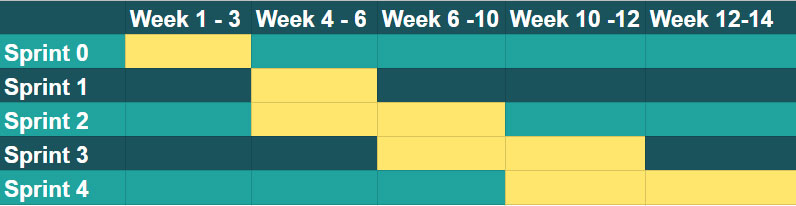
\includegraphics[scale = 0.5]{schedule.jpg}\\[1 cm]\cite{projectcolors}

\subsubsection{Sprint 0}

The name SPRINT 0 has been learned to describe the preparation phase which precedes the launching of the project. The term SPRINT 0 is being simpler to use than the preparation or inception phase, it is increasingly used in SCRUM projects.
Sprint 0 does not diminish the flexibility of our project. On the contrary, it will allow us to anticipate certain actions and have an overview that will facilitate the management of changes that  will emerge at the following sprints. \cite{DESTREMAU}

In this Sprint we will be able to  :
\begin{enumerate}
\item Share a clear vision of the project;
\item Identify users need;
\item Identify the preliminary workload resulting of the users need;
\item Prepare the project management plan;
\end{enumerate}
 
\subsubsection{Sprint 1}
The preliminary specification of the workload  in sprint 0
will help us in this sprint in modeling our data warehouse,thus the formalization of the entire workload.
In addition, in this phase it is essential to maintain an active technological watch to choose our Essential BI tools
used in  next sprints.
\subsubsection{Sprint 2}
In this sprint we will be able to define our data warehouse 's architecture, assess the  data quality and implement the designed ETL system.
\subsubsection{Sprint 3}
In this sprint we will be able to visualize our data using the BI restitution tools .
\subsubsection{Sprint 4}
In this final sprint , We will be able to prepare an oral
presentation where we summarize all the steps that we have gone through when developing our project 's data warehouse and present 
our work to our professors.

\subsection{Kanban}

In addition of Scrum methodology we choose to use Kanban approach, that means “visual card” in Japanese, to help us simplify the sprints workload. We going to make a visual work-flow using Trello for create and manage all cards with micro tasks, it will result in each sprints deliveries milestones. 

\subsubsection{Trello}
Trello\cite{trello} is a project management software that utilizes the concept of boards to represent
projects and within boards, cards to represent tasks. Trello supports Team Collaboration
enabling members to discuss a project in real-time. It keeps everybody informed through
task assignments, activity log, and e-mail notifications.\cite{tutorialspoint}



\section{Preliminary Workload}

\subsection{Data Sources}

The main services of stream nowadays are responsible for creating an efficient way to capture data and generate real information about the customers with it, but to obtain the success in this new world where data is like gold, they need to provide a service that is capable to get users loyalty. For this reason companies and communities of independent artists are building continuously distinct forms of technologies to present not only songs, but music with value add on it, such as, variety, quality and shareability. As a result of this frequent process innovation, today It's possible for any person to have access to huge an open-sources databases about music subjects. Hence,to make decisional projects become more simple with the follow assets MusicBrainz encyclopedia\cite{musicbrainz} and Spotify Web API. We choose to use into our project these datasets and, if necessary, others data sources could be attached as a asset during this project.\\

MusicBrainz Database\cite{musicbrainz} includes information about artists, release groups, releases, recordings,
works, and labels, as well as the many relationships between them [table \ref{table:1}].
It is a community-maintained open source encyclopedia of music information. This means that anyone can help contribute to the project by adding information about your favorite artists and their related works.The entire dataset is 1.8 GB.
\begin{table}[h!]
\begin{center}
 \begin{tabular}{||c c c ||} 
 \hline
 Attributes & type & granularity \\ [0.5ex] 
 \hline\hline
 released songs & text & by title \\ 
 \hline
 location & text & by region, country  \\
 \hline
 genre & text & by binary  \\
 \hline
 date & timestamp & by month,year  \\
 \hline
 artists & text & by name, alias  \\
 \hline
 origins & text & by country  \\
 \hline
 cover & text & by name  \\
 \hline
\end{tabular}
\caption{A brief description of MusicBrainz Database 's attributes.}
\label{table:1}
\end{center}
\end{table}

%, Lastfm & Million Song Dataset\cite{lastfm}
%Lastfm and Million Song Dataset\cite{lastfm} is a freely-available collection of audio features and metadata for a million contemporary popular music tracks.\\

Spotify Web API \cite{spotify} Based on simple REST principles, the Web API endpoints return metadata about music artists, albums, and tracks[table \ref{table:2}], directly from the Spotify Data Catalogue.
\begin{table}[h!]
\begin{center}
 \begin{tabular}{||c c c ||} 
 \hline
 Attributes & type & granularity \\ [0.5ex] 
 \hline\hline
 popularity & number & 0-100 \\ 
 \hline
 energy & float & 0.0 to 1.0  \\
 \hline
  valence & float & 0.0 to 1.0  \\
 \hline
 genre & text & by binary  \\
 \hline
 danceability & float & 0.0 to 1.0  \\
 \hline
 duration & number & by by milliseconds  \\
 \hline
 loudness & float & by decibels (dB) \\
 \hline
 mode & int & by major, minor \\
  \hline
 tempo & float & by beats per minute (BPM)\\
 \hline
\end{tabular}
\caption{A brief description of Spotify Web API 's attributes.}
\label{table:2}
\end{center}
\end{table}


\newpage

\subsection{User Needs}
Statistics about songs and artists:
\begin{itemize}
\item Number and Average of  released songs disaggregating by genre, year , location and artist .
\item The biggest/ lowest number of released songs by location , genre , year and artist .
\item Number of  artists disaggregating by origins.
\item Number of artists appeared every year in the music industry.
\item Number of songs or artists that achieved a certain popularity.
\item The average popularity of the songs where artists participated to analyze artist's performance.
\item What is the less popular songs by country and find out why ?
\item What is the impact of cover art on success of an album?
Number of  recorded covers disaggregating  by artist and song .
\item The most covered songs by artist and song  .
\item Artists that are most engaged in the last years.
\item What makes a  top performer based on songs ‘s technical features?
\end{itemize}
Statistics about song musical features:
\begin{itemize}
\item Average duration, average tempo by artist and/or location and/or year.
\item What makes a tube based on culture, market, political time, features of the song or the category of the song.
\end{itemize}


\section{Data Warehouse Modelling }
\subsection{Conceptual Design}
Conceptual modeling is widely recognized to be the necessary foundation for building a database that
is well-documented and fully satisfies the user requirements. In particular, from the designer point of
view the availability of a conceptual model provides a higher level of abstraction in describing the
warehousing process and its architecture in all its aspects. 
~\par For modelling our data warehouse schema we used The Dimensional Fact Model or DFM which is a graphical conceptual model, specifically devised for multidimensional design.
In subsection 4.2.1 , we present our conceptual models corresponding to our proposed fact schemas .
\subsubsection{Conceptual Schemas}
In order to represent our DFM models , we used the requirement-based design approach. It is a bottom-up technique that allowed us to do the mapping between our analyzed requirements in subsection 3.2 onto our available data source so that we get to locate the conceptual objects at sources and make sure that the data verifying our user needs effectively exists.
~\par Using this approach , We first start by defining the set of facts , measures and finally dimensions.
Figure 1 shows the fact schema for the analysis of songs and artists musical features in which the fact consists of a released song with all its features in the month ,city of release ,the song 's genre and the group artist that released the song .
%fact song picture
\begin{figure}[h]
    \centering
    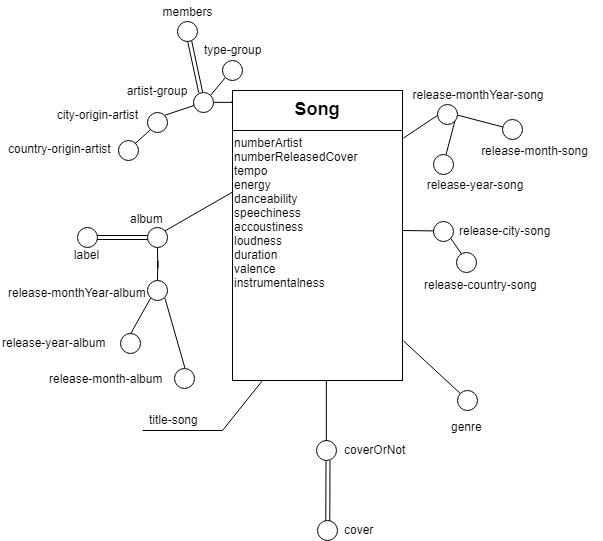
\includegraphics[scale =0.5]{fct-song.jpg}\\[1 cm]
    \caption{The Dimension Fact model for song.}
    \label{fig:factSong}
\end{figure}
\newpage
Figure 2 and 3 shows the fact schema for the analysis of songs and artists popularity in the which the fact consists of song's popularity (figure 2) and the artist 's popularity (figure3)
in every month .
%fact song Popularity picture
\begin{figure}[h]
    \centering
    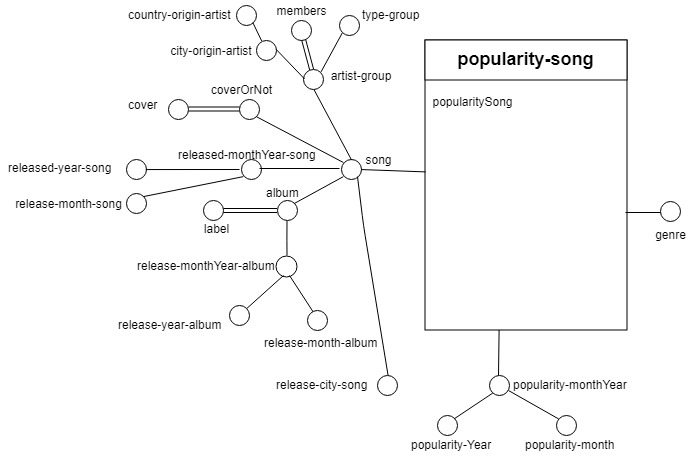
\includegraphics[scale =0.5]{fct-popularity-song.jpg}\\[1 cm]
    \caption{The Dimension Fact model for song popularity.}
    \label{fig:factPopularitySong}
\end{figure}

%fact artist Popularity picture
\begin{figure}[h]
    \centering
    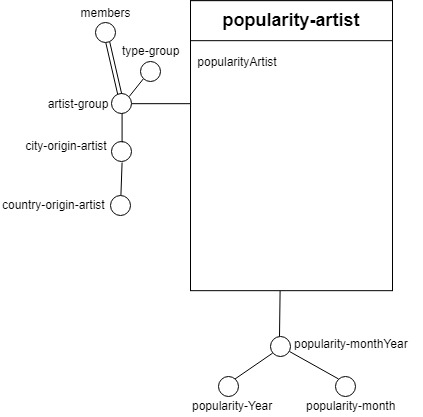
\includegraphics[scale =0.5]{fct-popularity-artist.jpg}\\[1 cm]
    \caption{The Dimension Fact model for artist popularity.}
    \label{fig:factPopularityArtist}
\end{figure}

\FloatBarrier

\subsubsection{Additivity Matrix}
In the additivity matrix we identify all the aggregation functions applied on measures and grouped by dimensions .
~\par Table 3 shows the equivalent additivity matrix for the fact schema in figure 1.
\begin{table}[h!]
\begin{center}
% l - left
% c - center
% r - right
% p - parameter ( i guess )
\begin{tabular}{@{}|p{4cm}|p{1cm}|p{2cm}|p{2cm}|p{1cm}|@{}}
\toprule
 & \multicolumn{1}{l|}{Group-artist} & Release-year-song & Release-city-song & genre\\ \midrule
numberArtist &  & Avg & \begin{tabular}[c]{@{}l@{}} Sum\\Avg
\end{tabular}{} & \begin{tabular}[c]{@{}l@{}} Sum \\Avg
\end{tabular}{} \\ \midrule
numberReleasedCover & \begin{tabular}[c]{@{}l@{}}  Max \\Avg
\end{tabular}{}   &Avg  &Avg  &   \\ \midrule
numberSong & \begin{tabular}[c]{@{}l@{}}  Max\\ Min\end{tabular}  & \begin{tabular}[c]{@{}l@{}} Avg\\ Max\\ Min\end{tabular} & \begin{tabular}[c]{@{}l@{}} Avg\\ Max\\ Min\end{tabular} & \begin{tabular}[c]{@{}l@{}} Avg\\ Max\\ Min\end{tabular}   \\ \midrule
tempo & Avg & Avg & Avg & Avg  \\ \midrule
energy & Avg  & Avg & Avg & Avg \\ \midrule
danceability & Avg  & Avg & Avg & Avg  \\ \midrule
speechiness & Avg  & Avg & Avg & Avg   \\ \midrule
accoustiness & Avg  & Avg & Avg & Avg   \\ \midrule
loudness & Avg & Avg & Avg & Avg   \\ \midrule
duration & Avg  & Avg & Avg & Avg   \\ \midrule
valence & Avg  & Avg & Avg & Avg   \\ \midrule
instrumentalness & Avg & Avg & Avg & Avg  \\ \bottomrule
\end{tabular}
\caption{Additivity matrix for Fact song.}
\end{center}
\end{table}
\FloatBarrier
Table 4 shows the equivalent additivity matrix for the fact schema in figure 2.
\begin{table}[h!]
\begin{center}
\begin{tabular}{|l|l|l|l|l|}
\hline
 & Song & Popularity-month & Group-artist & Popularity-year\\ \hline
popularitySong & \begin{tabular}[c]{@{}l@{}}Min\\ Max \\ Avg \end{tabular} & \begin{tabular}[c]{@{}l@{}}Min\\ Max \\ Avg \end{tabular} & \begin{tabular}[c]{@{}l@{}}Min\\ Max \\ Avg \end{tabular} 
& \begin{tabular}[c]{@{}l@{}}Min\\ Max \\ Avg \end{tabular} \\ \hline
\end{tabular}

\caption{Additivity matrix for Fact Popularity-Song .}
\end{center}
\end{table}
\FloatBarrier
Table 5 shows the equivalent additivity matrix for the fact schema in figure 3.
\begin{table}[h!]
\begin{center}
\begin{tabular}{@{}|l|l|l|l|@{}}
\toprule
 & Group-artist & Popularity-month &popularity-Year \\ \midrule
popularityArtist & \begin{tabular}[c]{@{}l@{}}Min \\ Max \\Avg \end{tabular} & \begin{tabular}[c]{@{}l@{}}Min \\ Max \\ Avg\end{tabular} & \begin{tabular}[c]{@{}l@{}}Min \\ Max \\Avg \end{tabular}\\ \bottomrule
\end{tabular}
\caption{Additivity matrix for Fact Popularity-Artist .}
\end{center}
\end{table}
\FloatBarrier

%#######################################################
\subsubsection{Data Dictionary}

An important part of any software project is to be able to provide information in a clear and accessible way. For this purpose, to have, previously, a list with all of data variable names and description allow an efficient approach to have access to the definition of each metadata. It makes the action of manage different terminologies, formats and contents less painful for the team and users.

For this reason we created a dictionary that contents all of our attributes names, the respective description and if it is a measure (M), dimension (D) or attribute descriptive (AD). Some description was imported from origin sources, however we made some changes to make more clear each attributes denotation.

%############ START OF THE FIRST PIECE OF THIS TABLE
\begin{table}[h!]
\begin{center}
\begin{tabular}{@{}|l|p{7cm}|c|c|c|@{}} 
\toprule
Attributes & Description & M & D & AD \\ [0.5ex] \midrule
release-monthYear-song & month and year number of the first song release. e.g. "082018" ("MMYYYY" - timestamp).& no & yes & no \\ \hline
release-month-song & month number of the first song release. e.g. "08" ("MM" - timestamp).& no & yes & no \\ \hline
%-------------------------------------------->
release-year-song & year number (e.g. "2018") of the first song release ( "YYYY" - timestamp). & no & yes & no \\ \bottomrule \midrule
%-------------------------------------------->
\end{tabular}
\caption{Data dictionary for dimensions, attributes and measures.}
\label{table:2}
\end{center}
\end{table}
%############ END OF THE FIRST PIECE OF THIS TABLE
%############ START OF THE SECOND PIECE OF THIS TABLE
\begin{table}[h!]
\begin{center}
\begin{tabular}{@{}|l|p{7cm}|c|c|c|@{}} 
\toprule
Attributes & Description & M & D & AD \\ [0.5ex] \midrule
%-------------------------------------------->
artist-group & it could be a solo singer (e.g. "Drake"), group (e.g."AC DC") or lineup (e.g. "Zedd, Maren Morris and Grey") that the release is primarily credited (string). & no & yes & no \\ \hline
%-------------------------------------------->
type-group & it represent the type of a group of musicians (e.g. band, orchestra) or an artist (e.g. solo) (string). & no & yes & no \\ \hline
%-------------------------------------------->
members & it could be a list of band members e.g. the current members of AC DC are Angus Young, Chris Slade, Stevie Young and W. Axl Rose (string). & no & yes & no \\ \bottomrule
%-------------------------------------------->
city-origin & origin city of an artist or a band e.g. "Liverpool"(string). & no & yes & no \\ \hline
%-------------------------------------------->
country-origin & origin country of an artist or a band e.g. "United Kingdom" (string).  & no & yes & no \\ \hline
%-------------------------------------------->
numberArtist & is a measure to known the number of artists in a group or band, even in a solo arrangement. If artist-group is composed of one artist e.g. "Lady Gaga", numberArtist takes 1 as a value. & yes & no & no \\ \hline
%-------------------------------------------->
numberSong & an integer measure to know how many songs a group artist have released . & yes & no & no \\ \bottomrule \midrule
%-------------------------------------------->
title-song & a string that contains a music name or a title of a release e.g. "La corrida" . & no & no & no \\ \hline
%-------------------------------------------->
album & is a string with the album name e.g. "Samedi soir sur la Terre" & no & yes & yes \\ \hline
%-------------------------------------------->
label & the label which issued the release. There may be more than one for every released song , e.g. imprint, record company, music group, others (string). & no & yes & yes \\ \hline
%-------------------------------------------->
release-month-album & month of the first release of the album(e.g. "April", in timestamp)  & no & yes & no \\ \hline
%-------------------------------------------->
release-year-album & year of the first release of the album(e.g. "YYYY", in timestamp). & no & yes & no \\ \bottomrule \midrule
%-------------------------------------------->
\end{tabular}
\caption{Data dictionary for dimensions, attributes and measures.}
\label{table:2}
\end{center}
\end{table}
%############ END OF THE FIRST PIECE OF THIS TABLE
%############ START OF THE SECOND PIECE OF THIS TABLE
\begin{table}[h!]
\begin{center}
\begin{tabular}{@{}|l|p{7cm}|c|c|c|@{}} 
\toprule
Attributes & Description & M & D & AD \\ [0.5ex] \midrule
%-------------------------------------------->
cover & is artist, lineup or band that make a new performance or recording of a song that already exists, e.g. Andrei Zevakin, Ariadne and Martti Hallik. & no & yes & no \\ \hline
%-------------------------------------------->
coverOrNot & a simple Boolean value to know whether a song has at least one related cover (or not at all). (0 to false, 1 to true) & no & yes & no \\ \hline
%-------------------------------------------->
numberReleasedCover & a measure to know how many times a song has covered by an  artist or group (Integer). & yes & no & no \\ \hline\hline
%-------------------------------------------->
release-city-song & release city of a song & no & yes & no \\ \hline
%-------------------------------------------->
release-country-song & release country of a song . & no & yes & no \\ \bottomrule \midrule
%-------------------------------------------->
genre & is the genre of the song. e.g. "Rock".The genre of the song usually inherited from the album 's genre. & no & yes & no \\ \bottomrule \midrule

%-------------------------------------------->
tempo & is a measure of speed or pace of a given piece and derives directly from the average beat per minute (BPM) duration e.g. Billie Jean have 92 BPM (integer). & yes & no & no \\ \hline
%-------------------------------------------->
energy & is a measure from 0.0 to 1.0 and represents a perceptual measure of intensity and activity, e.g. Cut To The Feeling has a energy 0.905 that means a high level of activity. Combined with others measure can suggest feelings. & yes & no & no \\ \hline
%-------------------------------------------->
danceability & is a measure that describes how suitable a track is for dancing based on a combination of musical elements including tempo, rhythm stability, beat strength, and overall regularity. A track closer to 0.0 is least danceable than a music near 1.0 that is most danceable, e.g. Cut To The Feeling has a 0.696 of danceability. & yes & no & no \\ \hline
%-------------------------------------------->
\end{tabular}
\caption{Data dictionary for dimensions, attributes and measures.}
\label{table:2}
\end{center}
\end{table}
%############ END OF THE FIRST PIECE OF THIS TABLE
%############ START OF THE SECOND PIECE OF THIS TABLE
\begin{table}[h!]
\begin{center}
\begin{tabular}{@{}|l|p{9cm}|c|c|c|@{}} 
\toprule
Attributes & Description & M & D & O \\ [0.5ex] \midrule
%-------------------------------------------->
speechiness & is a float measure that can detect the presence of spoken words in a track.The more exclusively speech-like the recording (e.g. talk show, audio book, poetry), the closer to 1.0 the attribute value. Values above 0.66 describe tracks that are probably made entirely of spoken words. Values between 0.33 and 0.66 describe tracks that may contain both music and speech, either in sections or layered, including such cases as rap music. Values below 0.33 most likely represent music and other non-speech-like tracks. & yes & no & no \\ \hline
%-------------------------------------------->
accoustiness & it is a float confidence measure from 0.0 to 1.0 of whether the track is acoustic, e.g. 1.0 represents high confidence the track is acoustic. & yes & no & no \\ \hline
%-------------------------------------------->
loudness & it is a float measure of a track in decibels (dB). Loudness values are averaged across the entire track and are useful for comparing relative noise into a track. It is the quality of a sound that is the primary psychological correlate of physical strength (amplitude). Values typical range between -60 and 0 db.  & yes & no & no \\ \hline
%-------------------------------------------->
duration & the duration of the track in milliseconds(Float). & yes & no & no \\ \hline
%-------------------------------------------->
valence & is a float measure from 0.0 to 1.0 describing the musical positiveness conveyed by a track. Tracks with high valence sound more positive (e.g. happy, cheerful, euphoric), while tracks with low valence sound more negative (e.g. sad, depressed, angry).  & yes & no & no \\ \hline
%-------------------------------------------->
instrumentalness & is a float measure that predicts whether a track contains no vocals. “Ooh” and “aah” sounds are treated as instrumental in this context. Rap or spoken word tracks are clearly “vocal”. The closer the instrumentalness value is to 1.0, the greater likelihood the track contains no vocal content. Values above 0.5 are intended to represent instrumental tracks, but confidence is higher as the value approaches 1.0. & yes & no & no \\ \bottomrule \midrule
%-------------------------------------------->
\end{tabular}
\caption{Data dictionary for dimensions, attributes and measures.}
\label{table:2}
\end{center}
\end{table}
%############ END OF THE FIRST PIECE OF THIS TABLE
%############ START OF THE SECOND PIECE OF THIS TABLE
\begin{table}[h!]
\begin{center}
\begin{tabular}{@{}|l|p{9cm}|c|c|c|@{}} 
\toprule
Attributes & Description & M & D & O \\ [0.5ex] \midrule
%-------------------------------------------->
song & it's a dimension that contains song 's features and name (of the song). & no & yes & no \\ \bottomrule \midrule
%-------------------------------------------->
popularity-month & the month that corresponds to the value of the popularity , e.g. september (timestamp). & no & yes & no \\ \hline
%-------------------------------------------->
popularity-year & the year that corresponds to the value of the popularity, e.g. 2017 ("YYYY" timestamp). & no & yes & no \\ \bottomrule \midrule
%-------------------------------------------->
popularitySong & is a measure that present popularity of the track. This value will be between 0 and 100, whether closer to 100 being is the most popular.
Songs that are being played a lot now will have a higher popularity than songs that were played a lot in the past. Duplicate tracks (e.g. the same track from a single and an album) are rated independently. & yes & no & no \\ \hline
%-------------------------------------------->
popularityArtist & is a measure that present popularity of the artist and album, however this popularity is derived mathematically from track popularity (popularitySong). & yes & no & no \\ \bottomrule \midrule
%-------------------------------------------->
\end{tabular}
\caption{Data dictionary for dimensions, attributes ans measures.}
\label{table:2}
\end{center}
\end{table}
\FloatBarrier
%#######################################################


\subsection{Formalization of Requirements }
In this section ,we tried to refine our workload by identifying queries that are expressed directly on the conceptual model in a formal language in order to validate our conceptual models.
\begin{itemize}
    %------------------------------------#
\item user need 1/2:
\begin{itemize}
\item SONG[genre,release-year-song,release-city-song,artist-group].
numberSong 
\end{itemize}

%------------------------------------#
\item user need 3:
\begin{itemize}
\item SONG[city-origin-artist].numberArtist 
\end{itemize}
%------------------------------------#
\item user need 4:
\begin{itemize}
\item SONG[release-year-song;title-song IN [title-song,release-year-song,artist-group,
Min(release-year-song)].title-song].numberArtist
\end{itemize}
%------------------------------------#
\item user need 5:
\begin{itemize}
\item POPULARITY-ARTIST[artist-group;popularity $>$ X].numberArtist
\item POPULARITY-SONG[title-song;popularity $>$ X].numberSong
\end {itemize}
%------------------------------------#
\item user need 6:
\begin{itemize}
\item POPULARITY-SONG[artist-group].popularitySong
 \end{itemize}
 %------------------------------------#
\item user need 7:
\begin{itemize}
\item POPULARITY-SONG[Song,release-country-song;\hfill \break
popularitySong=[POPULARITY-SONG[release-country-song].Min(popuaritySong)]
\end{itemize}
%------------------------------------#
\item user need 8:
\begin{itemize}
\item POPULARITY-SONG[coverOrNot].popularitySong
\item SONG[artist-group].numberReleasedCover
\end{itemize}
 %------------------------------------#
\item user need 9:
 \begin{itemize}
\item SONG[artist-group,title-song,coverOrNot=1].numberReleasedCover
\end{itemize}
%------------------------------------#
\item user need 10:
\begin{itemize}
\item SONG[artist-group,title-song].Max(numberReleasedCover)
\end{itemize}
%------------------------------------#
\item user need 11:
\begin{itemize}
\item SONG+POPULARITY-SONG[;popularity $>$ X].tempo
\item SONG+POPULARITY-SONG[;popularity $>$ X].energy
\end{itemize}
%------------------------------------#
\item user need 12:
\begin{itemize}
\item SONG[artist-group;release-year-song $>$= 2016 and  \hfill \break 
release-year-song $<$=2018].Max(numberSong)
\end{itemize}
%------------------------------------#
\item user need 13:
\begin{itemize}
\item SONG[artist-group,release-city-song,release-year-song].Avg(Duration)
\item SONG[artist-group,release-city-song,release-year-song].Avg(Tempo)
\end{itemize}
 %------------------------------------#
\item additional request 1: \hfill \break 
This query calculates the popularity of group artists in each month in 2016 and its members are six or less:
\begin{itemize}
\item Popularity-artist[month, groupArtist; year='2016', artist-group in SONG[year, artist-group; year = '2016' and numberArtist $<$= 6].artist-group].popularityArtist
\end{itemize}
\end{itemize}
\subsection{Prototypes of Charts}
\begin{figure}
    \centering
    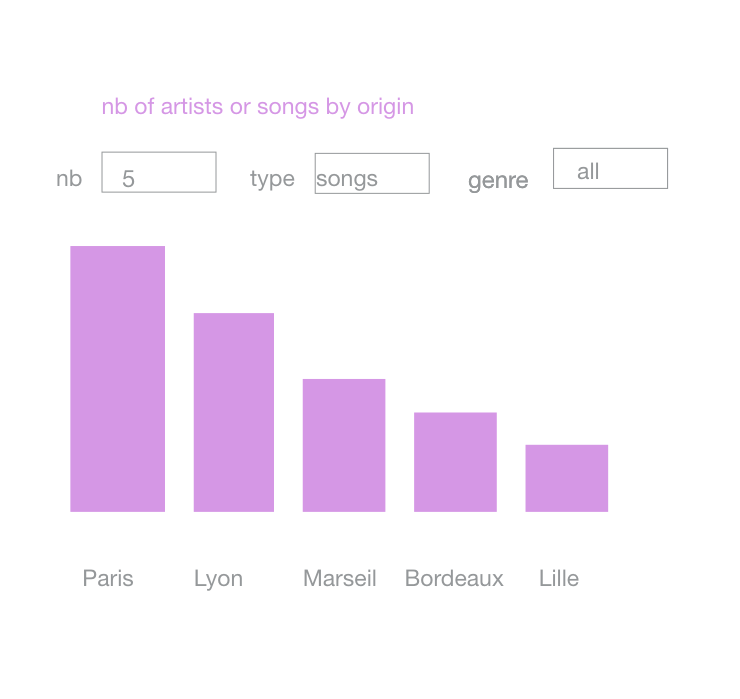
\includegraphics[height=13cm]{city.png}
    \caption{prototype of figure presenting the number of songs or artists by city}
    \label{fig:my_label}
\end{figure}
\begin{figure}
    \centering
    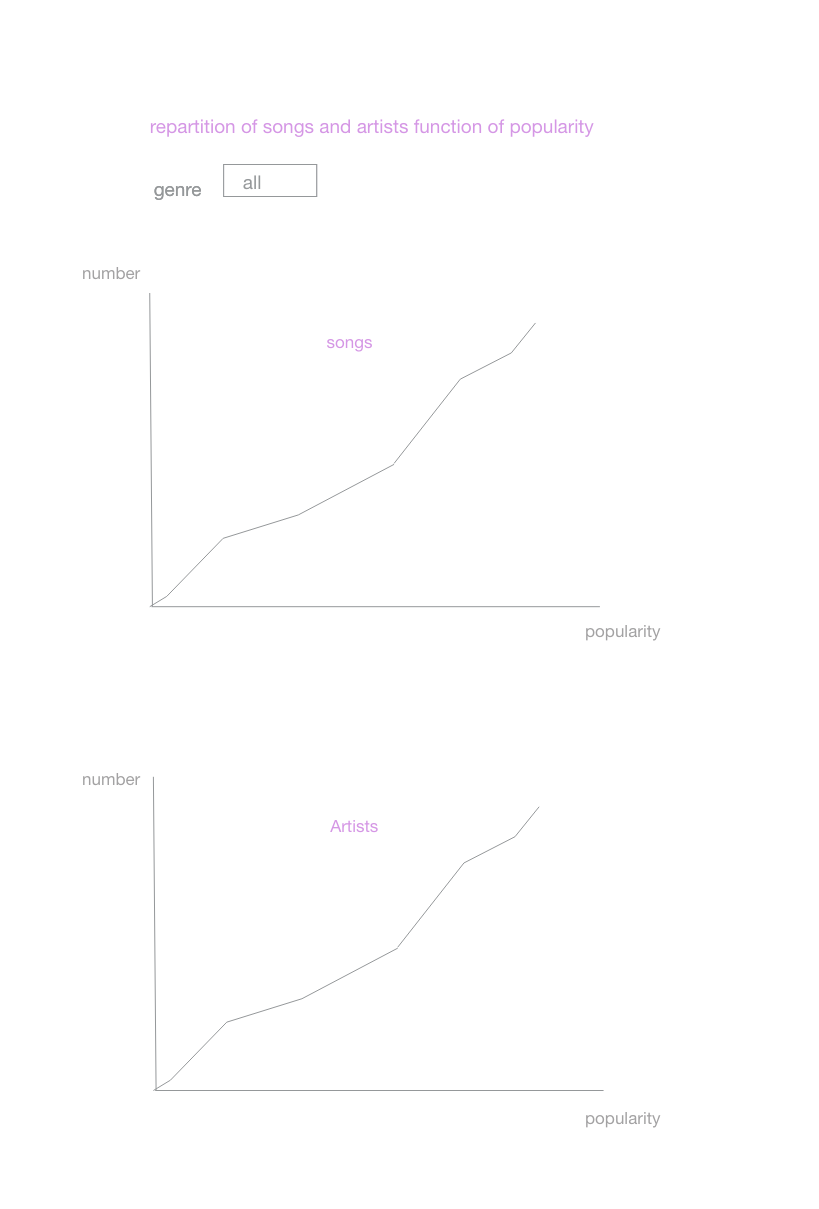
\includegraphics[height=13cm]{culukated.png}
    \caption{prototype of figure presenting the re-partition of artists and song function of popularity}
    \label{fig:my_label}
\end{figure}

\begin{figure}
    \centering
    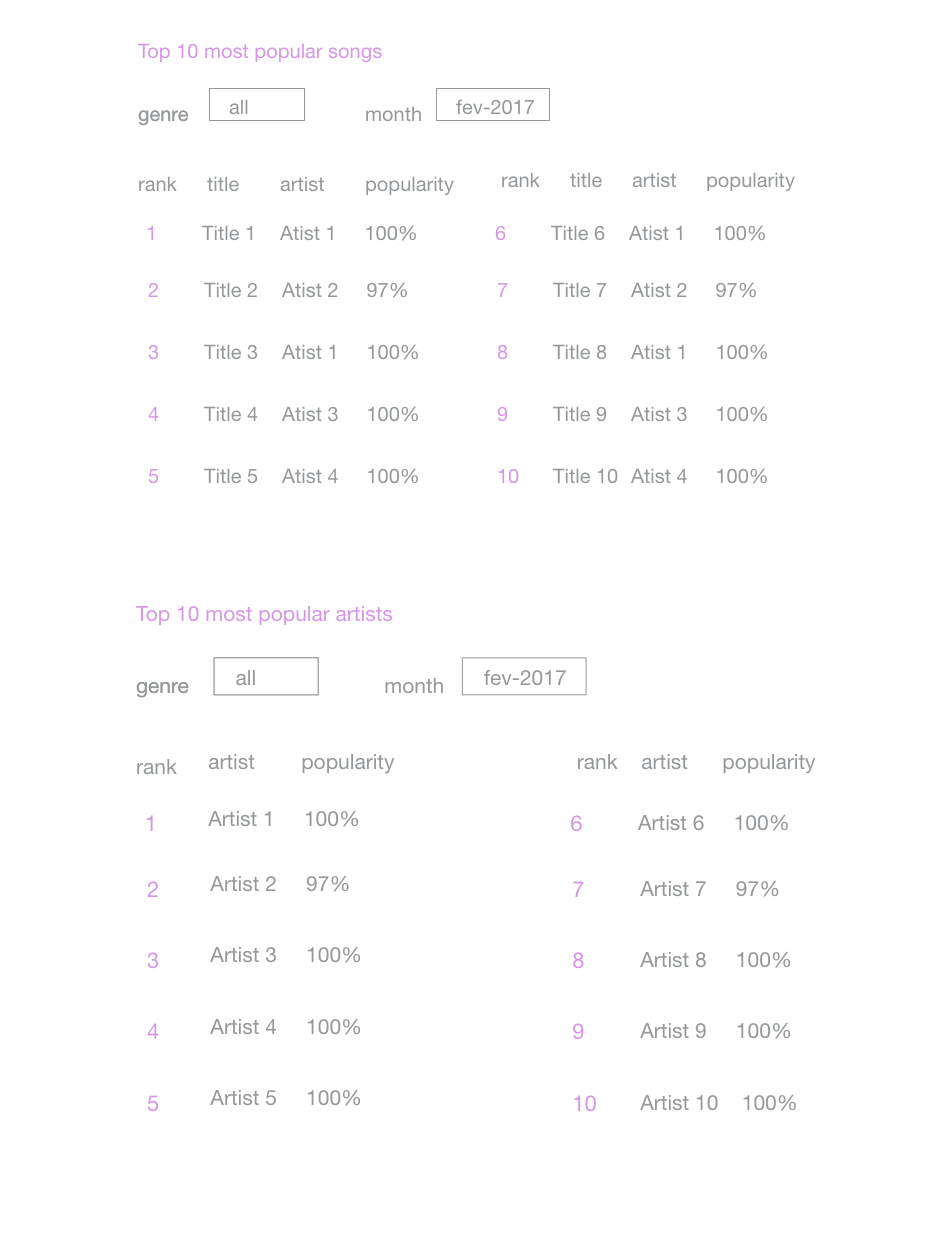
\includegraphics[height=13cm]{ranking.png}
    \caption{ranking of song and artist by popularity}
    \label{fig:my_label}
\end{figure}

\begin{figure}
    \centering
    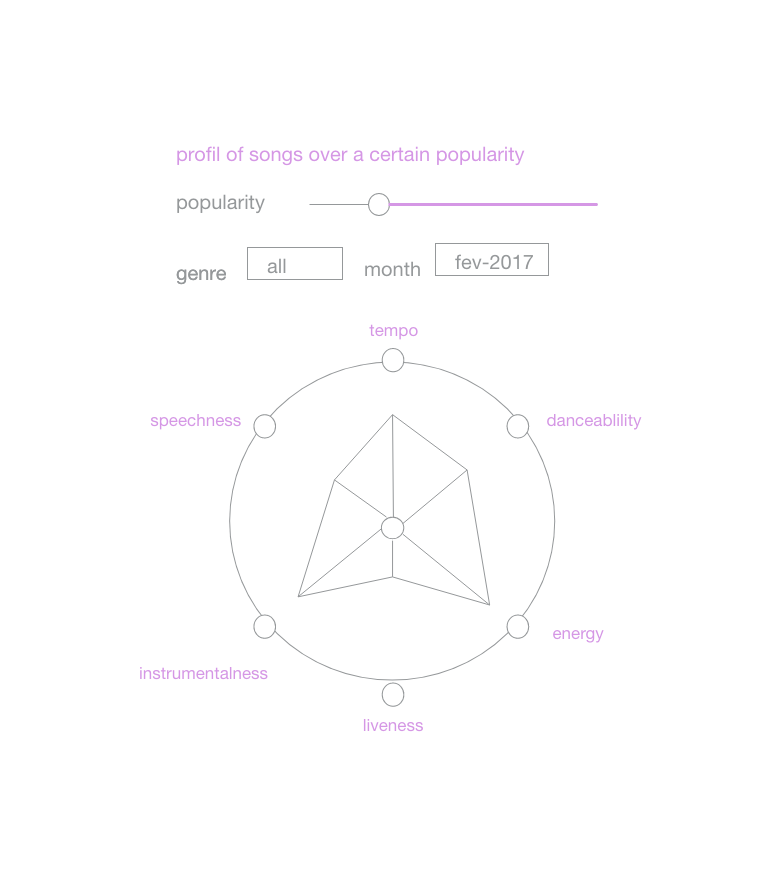
\includegraphics[height=13cm]{technical.png}
    \caption{prototype of figure presenting the average technical measures for songs over a certain popularity}
    \label{fig:my_label}
\end{figure}

\newpage
\bibliographystyle{plain}
\bibliography{biblist}

\end{document}